\documentclass[hidelinks,aspectratio=169]{beamer}
\usepackage[english]{babel} 
\usepackage[utf8]{inputenc} 
\usepackage{fourier} 

%Slide colors
\usetheme{Boadilla}
\usecolortheme{beaver}

% Images
\usepackage{graphicx}
\usepackage{caption}
\usepackage{subcaption}
\usepackage{float}
\graphicspath{ {../Images} }

% Stop hyphenation
\usepackage[none]{hyphenat}

% Coloring links
\usepackage{xcolor}

% Enumerate abc
\usepackage{enumerate}

% Minipages in the same line
\usepackage{tabularx}

% Redefines caption setup in way to remove "Figure:"
\usepackage{caption}
\captionsetup[figure]{labelformat=empty}

% Use for the matrix creation
\usepackage{amsmath}
\usepackage{array}
\usepackage{geometry}
\usepackage{bbding}
\usepackage{amssymb}

% License
\usepackage[
type={CC},
modifier={by-nc-sa},
version={4.0},
]{doclicense}

% Command to enumerate frames title
\newcommand{\numcirc}[1]{%
	\large
	\usebeamercolor[bg]{item projected}%
	\begin{pgfpicture}{-1ex}{0ex}{1ex}{2ex}
		\pgfpathcircle{\pgfpoint{0pt}{.75ex}}{1.2ex}
		\pgfusepath{fill}
		\pgftext[base]{\color{fg}#1}
	\end{pgfpicture}%
	\usebeamerfont*{frametitle}%
}

%Command to zoom in
\usepackage{mwe}
\makeatletter
\newsavebox\zb@x
\newcounter{z@@m}
\usepackage{calc}
\newdimen\B@r\newdimen\P@r
\newdimen\@zw\newdimen\@zh\newdimen\@zd

\newcommand{\zoombox}[2][0]{%
	\leavevmode%
	\sbox\zb@x{#2}%
	\setlength\B@r{1pt*\ratio{\wd\zb@x}{\ht\zb@x+\dp\zb@x}}%
	\setlength\P@r{1pt*\ratio{\paperwidth}{\paperheight}}%
	\ifdim\B@r>\P@r\relax%
	\setlength\@zw{\wd\zb@x}\setlength\@zh{\@zw*\ratio{\paperheight}{\paperwidth}}%
	\setlength\@zd{(\@zh-\ht\zb@x-\dp\zb@x)*\real{0.5}+\dp\zb@x}%
	\setlength\@zh{\@zh-\@zd}%
	\else%
	\setlength\@zh{\ht\zb@x+\dp\zb@x}%
	\setlength\@zw{\@zh*\ratio{\paperwidth}{\paperheight}}%
	\setlength\@zh{\ht\zb@x}\setlength\@zd{\dp\zb@x}%
	\fi%
	\makebox[0pt][l]{\makebox[\wd\zb@x][c]{\makebox[\@zw][l]{%
				\pdfdest name {zbfs\thez@@m} fitr
				width  \@zw\space
				height \@zh\space
				depth  \@zd\space
	}}}%
	\pdfdest name {zb\thez@@m} fitr
	width  \wd\zb@x\space
	height \ht\zb@x\space
	depth  \dp\zb@x\space
	\immediate\pdfannot 
	width  \wd\zb@x\space
	height \ht\zb@x\space
	depth  \dp\zb@x\space
	{%
		/Subtype/Link/H/N
		/Border [0 0 #1 [1 2]]
		/A <<
		/S/JavaScript
		/JS (
		if(typeof(zoomed)=='undefined'||!zoomed){
			var lastView=this.viewState;
			if(app.fs.isFullScreen) this.gotoNamedDest('zbfs\thez@@m');
			else this.gotoNamedDest('zb\thez@@m');
			zoomed=true;
		}else{
			this.viewState=lastView;
			zoomed=false;
		}
		)
		>>
	}%
	\usebox{\zb@x}%
	\stepcounter{z@@m}%
} 
\makeatother

%Setting Table of contents font size
\setbeamerfont{subsection in toc}{size=\small}

%Header
\title[BINARY CODE]{\textbf{BINARY CODE}}
\author{Francesco Rombaldoni}
\date{}

\begin{document}
	
	\begin{frame}
		\maketitle
		
		\vspace*{\fill}
		\centering
		\fboxrule=2pt
		\fbox
		{
			\begin{minipage}{0.9\linewidth}
				\small{This document is optimized for digital viewing with \href{https://get.adobe.com/reader/}{\textcolor{blue}{Adobe~Acrobat~Reader}}.}  
			\end{minipage}
		}
	\end{frame}
	
	\begin{frame}
		\tableofcontents
	\end{frame}
	
	\section{\textbf{What is binary code?}}
	\begin{frame}{\textbf{What is binary code?}}
		\begin{center}
			\begin{itemize}
				\item To count and do simple calculations, we usually use the classic decimal system with the ten digits from 0 to 9.\\
				To count and do complicated calculations, computers use a different system called the \textbf{binary system}, because it is made up of only two symbols: 0 and 1.
			\end{itemize}
			\vspace*{0.5cm}
			\begin{itemize}
				\item Computers only understand these two symbols because they either receive a signal or not, so:
				\begin{itemize}
					\item \textbf{0}, which means no signal (so 0 $\rightarrow$ off)
					\item \textbf{1}, which means there is voltage (so 1 $\rightarrow$ on)
				\end{itemize}
			\end{itemize}
		\end{center}
		\vspace*{0.5cm}
		\begin{center}
			\begin{itemize}
				\item \hspace*{5cm}\textbf{0 $\rightarrow$ OFF}
				\item \hspace*{5cm}\textbf{1 $\rightarrow$ ON}
			\end{itemize}
		\end{center}
	\end{frame}
	
	\section{\textbf{Try to understand}}
	\begin{frame}{\textbf{Try to understand}}
		\begin{tabularx}{\textwidth}{XXX}
			{
				\begin{tabularx}{0.3\textwidth}{XX}
					{
						\zoombox{
\includegraphics[scale=0.22]{black_lamp.png}}
					}&{
						\zoombox{
\includegraphics[scale=0.22]{black_lamp.png}}
					}
				\end{tabularx}
				
				\begin{tabularx}{0.3\textwidth}{XX}
					{
						\zoombox{
\includegraphics[scale=0.22]{black_lamp.png}}
					}&{
						\hspace*{-1mm}\zoombox{
\includegraphics[scale=0.17]{light_lamp.png}}
					}	
				\end{tabularx}
				
				\begin{tabularx}{0.3\textwidth}{XX}
					{
						\hspace*{-1mm}\zoombox{
\includegraphics[scale=0.17]{light_lamp.png}}
					}&{
						\hspace*{-1mm}\zoombox{
\includegraphics[scale=0.17]{light_lamp.png}}
					}
				\end{tabularx}
			}&{
			
				\vspace*{-2cm}
			
				\begin{center}
					
					\zoombox{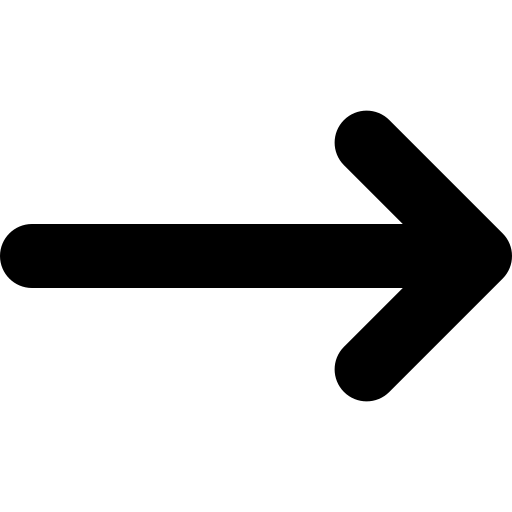
\includegraphics[width=5cm,height=2cm]{right_arrow.png}}
					
					\zoombox{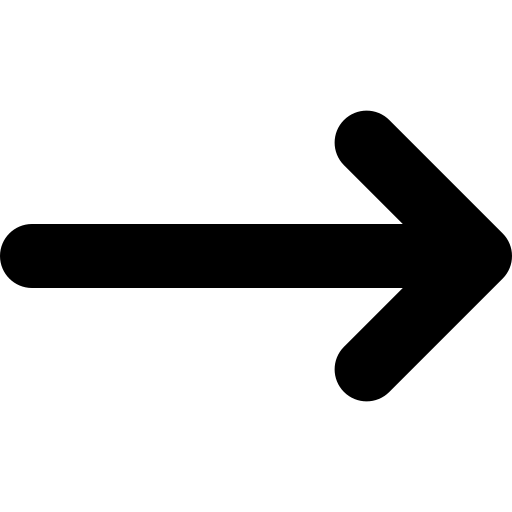
\includegraphics[width=5cm,height=2cm]{right_arrow.png}}
					
					\zoombox{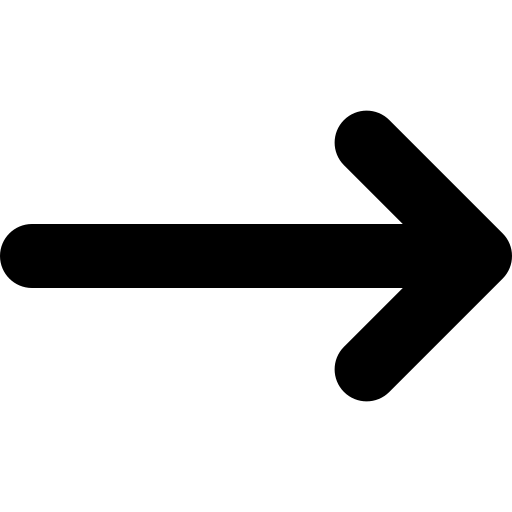
\includegraphics[width=5cm,height=2cm]{right_arrow.png}}
					
				\end{center}
			
			}&{
			
					\hspace*{1cm}
					\begin{tabularx}{0.3\textwidth}{XX}
						{	\vspace*{-0.8cm}
							\textbf{\huge 0}
						}&{
							\vspace*{-0.8cm}
							\textbf{\huge 0}
						}
					\end{tabularx}
						
					\hspace*{1cm}
					\begin{tabularx}{0.3\textwidth}{XX}
						{
							\vspace*{0.8cm}
							\textbf{\huge 0}
						}&{
							\vspace*{0.8cm}
							\textbf{\huge 1}
						}
					\end{tabularx}
					
					\hspace*{1cm}
					\begin{tabularx}{0.3\textwidth}{XX}
					{
						\vspace*{1cm}
						\textbf{\huge 1}
					}&{
						\vspace*{1cm}
						\textbf{\huge 1}
					}
					\end{tabularx}
			}
		\end{tabularx}
	\end{frame}
	
	\section{\textbf{So what?}}
	\begin{frame}{\textbf{So what?}}
		\begin{itemize}
			\item Using only these two digits, you can represent not only all possible numbers, but also all words, pictures, videos, sounds... all kinds of digital things.
		\end{itemize}
		\begin{center}
			\[
			\scalebox{1.5}{
				$\begin{bmatrix}
					0 & 1 & 0 & 1 & 1 & 0 & 0 & 1 \\
					1 & 0 & 1 & 0 & 1 & 1 & 0 & 0 \\
					0 & 0 & 1 & 1 & 0 & 1 & 1 & 0 \\
					1 & 1 & 0 & 0 & 1 & 0 & 1 & 1 \\
					0 & 1 & 1 & 0 & 0 & 1 & 0 & 1 \\
				\end{bmatrix}$
			}
			\]
		\end{center}
	\end{frame}
	
	
	\section{\textbf{Think about your name in binary code!}}
	\begin{frame}{\textbf{Think about your name in binary code!}}
		\renewcommand{\arraystretch}{1}
		\centering
		\begin{tabular}{|c|>{\ttfamily}c|c|>{\ttfamily}c|}
			\hline
			\textbf{Letter} & \textbf{ASCII Binary} & \textbf{Letter} & \textbf{ASCII Binary} \\
			\hline
			\textbf{A} & 01000001 & \textbf{N} & 01001110 \\
			\textbf{B} & 01000010 & \textbf{O} & 01001111 \\
			\textbf{C} & 01000011 & \textbf{P} & 01010000 \\
			\textbf{D} & 01000100 & \textbf{Q} & 01010001 \\
			\textbf{E} & 01000101 & \textbf{R} & 01010010 \\
			\textbf{F} & 01000110 & \textbf{S} & 01010011 \\
			\textbf{G} & 01000111 & \textbf{T} & 01010100 \\
			\textbf{H} & 01001000 & \textbf{U} & 01010101 \\
			\textbf{I} & 01001001 & \textbf{V} & 01010110 \\
			\textbf{J} & 01001010 & \textbf{W} & 01010111 \\
			\textbf{K} & 01001011 & \textbf{X} & 01011000 \\
			\textbf{L} & 01001100 & \textbf{Y} & 01011001 \\
			\textbf{M} & 01001101 & \textbf{Z} & 01011010 \\
			\hline
		\end{tabular}
	\end{frame}
	
	\section{\textbf{Translating a sentence}}
	\begin{frame}{\textbf{Translating a sentence}}
		\begin{center}
			\textbf{\huge GOOD LUCK!}
		\end{center}
		\vspace*{0.5cm}
		\begin{center}
			\renewcommand{\arraystretch}{1.5}
			% First table: GOOD
			\begin{tabular}{|>{\centering\arraybackslash}m{2cm}|>{\centering\arraybackslash}m{2cm}|>{\centering\arraybackslash}m{2cm}|>{\centering\arraybackslash}m{2cm}|}
				\hline
				\textbf{G} & \textbf{O} & \textbf{O} & \textbf{D} \\
				\hline
				01000111 & 01001111 & 01001111 & 01000100 \\
				\hline
			\end{tabular}
			
			\vspace{1cm} % vertical space between tables
			
			% Second table: LUCK!
			\begin{tabular}{|>{\centering\arraybackslash}m{1.6cm}|>{\centering\arraybackslash}m{1.6cm}|>{\centering\arraybackslash}m{1.6cm}|>{\centering\arraybackslash}m{1.6cm}|>{\centering\arraybackslash}m{1.6cm}|}
				\hline
				\textbf{L} & \textbf{U} & \textbf{C} & \textbf{K} & \textbf{!} \\
				\hline
				01001100 & 01010101 & 01000011 & 01001011 & 00100001 \\
				\hline
			\end{tabular}
		\end{center}
	\end{frame}
	
	\section{\textbf{Translating a word}}
	\begin{frame}{\textbf{Translating a word}}
		\begin{center}
			\textbf{\huge HELLO}
		\end{center}
		\vspace*{0.5cm}
		\begin{center}
			\renewcommand{\arraystretch}{1.5}
			\begin{tabular}{|>{\centering\arraybackslash}m{2.2cm}|>{\centering\arraybackslash}m{2.2cm}|>{\centering\arraybackslash}m{2.2cm}|>{\centering\arraybackslash}m{2.2cm}|>{\centering\arraybackslash}m{2.2cm}|}
				\hline
				\textbf{H} & \textbf{E} & \textbf{L} & \textbf{L} & \textbf{O} \\
				\hline
				01001000 & 01000101 & 01001100 & 01001100 & 01001111 \\
				\hline
			\end{tabular}
		\end{center}
	\end{frame}
	
\section{\textbf{Not just 0 and 1}}
\begin{frame}{\textbf{Not just 0 and 1}}
	\renewcommand{\arraystretch}{1}
	\centering
	\begin{tabular}{|c|c|c|c|}
		\hline
		\textbf{Letter} & \textbf{Binary code (squares)} & \textbf{Letter} & \textbf{Binary code (squares)} \\
		\hline
		\textbf{A} & $\blacksquare\square\blacksquare\blacksquare\blacksquare\blacksquare\blacksquare\square$ & \textbf{N} & $\blacksquare\square\blacksquare\square\square\blacksquare\blacksquare\square$ \\
		\textbf{B} & $\blacksquare\square\blacksquare\blacksquare\blacksquare\blacksquare\square\square$ & \textbf{O} & $\blacksquare\square\blacksquare\square\square\blacksquare\blacksquare\blacksquare$ \\
		\textbf{C} & $\blacksquare\square\blacksquare\blacksquare\blacksquare\square\blacksquare\square$ & \textbf{P} & $\blacksquare\square\blacksquare\square\blacksquare\blacksquare\blacksquare\blacksquare$ \\
		\textbf{D} & $\blacksquare\square\blacksquare\blacksquare\blacksquare\square\square\square$ & \textbf{Q} & $\blacksquare\square\blacksquare\square\blacksquare\blacksquare\square\square$ \\
		\textbf{E} & $\blacksquare\square\blacksquare\blacksquare\blacksquare\square\blacksquare\blacksquare$ & \textbf{R} & $\blacksquare\square\blacksquare\square\blacksquare\blacksquare\square\blacksquare$ \\
		\textbf{F} & $\blacksquare\square\blacksquare\blacksquare\blacksquare\square\square\blacksquare$ & \textbf{S} & $\blacksquare\square\blacksquare\square\blacksquare\square\blacksquare\square$ \\
		\textbf{G} & $\blacksquare\square\blacksquare\square\blacksquare\blacksquare\blacksquare\square$ & \textbf{T} & $\blacksquare\square\blacksquare\square\blacksquare\square\blacksquare\blacksquare$ \\
		\textbf{H} & $\blacksquare\square\blacksquare\square\blacksquare\blacksquare\square\square$ & \textbf{U} & $\blacksquare\square\blacksquare\square\square\blacksquare\square\square$ \\
		\textbf{I} & $\blacksquare\square\blacksquare\square\square\blacksquare\blacksquare\square$ & \textbf{V} & $\blacksquare\square\blacksquare\square\square\blacksquare\square\blacksquare$ \\
		\textbf{J} & $\blacksquare\square\blacksquare\square\square\square\blacksquare\square$ & \textbf{W} & $\blacksquare\square\blacksquare\square\square\square\blacksquare\blacksquare$ \\
		\textbf{K} & $\blacksquare\square\blacksquare\square\blacksquare\blacksquare\blacksquare\square$ & \textbf{X} & $\blacksquare\square\blacksquare\square\square\square\square\square$ \\
		\textbf{L} & $\blacksquare\square\blacksquare\square\blacksquare\blacksquare\square\blacksquare$ & \textbf{Y} & $\blacksquare\square\blacksquare\square\square\square\square\blacksquare$ \\
		\textbf{M} & $\blacksquare\square\blacksquare\square\square\blacksquare\blacksquare\square$ & \textbf{Z} & $\blacksquare\square\blacksquare\square\square\square\blacksquare\square$ \\
		\hline
	\end{tabular}
\end{frame}

\section{\textbf{Make a bracelet with the initials of your name}}
\begin{frame}{\textbf{Make a bracelet with the initials of your name}}
	\begin{center}
		\zoombox{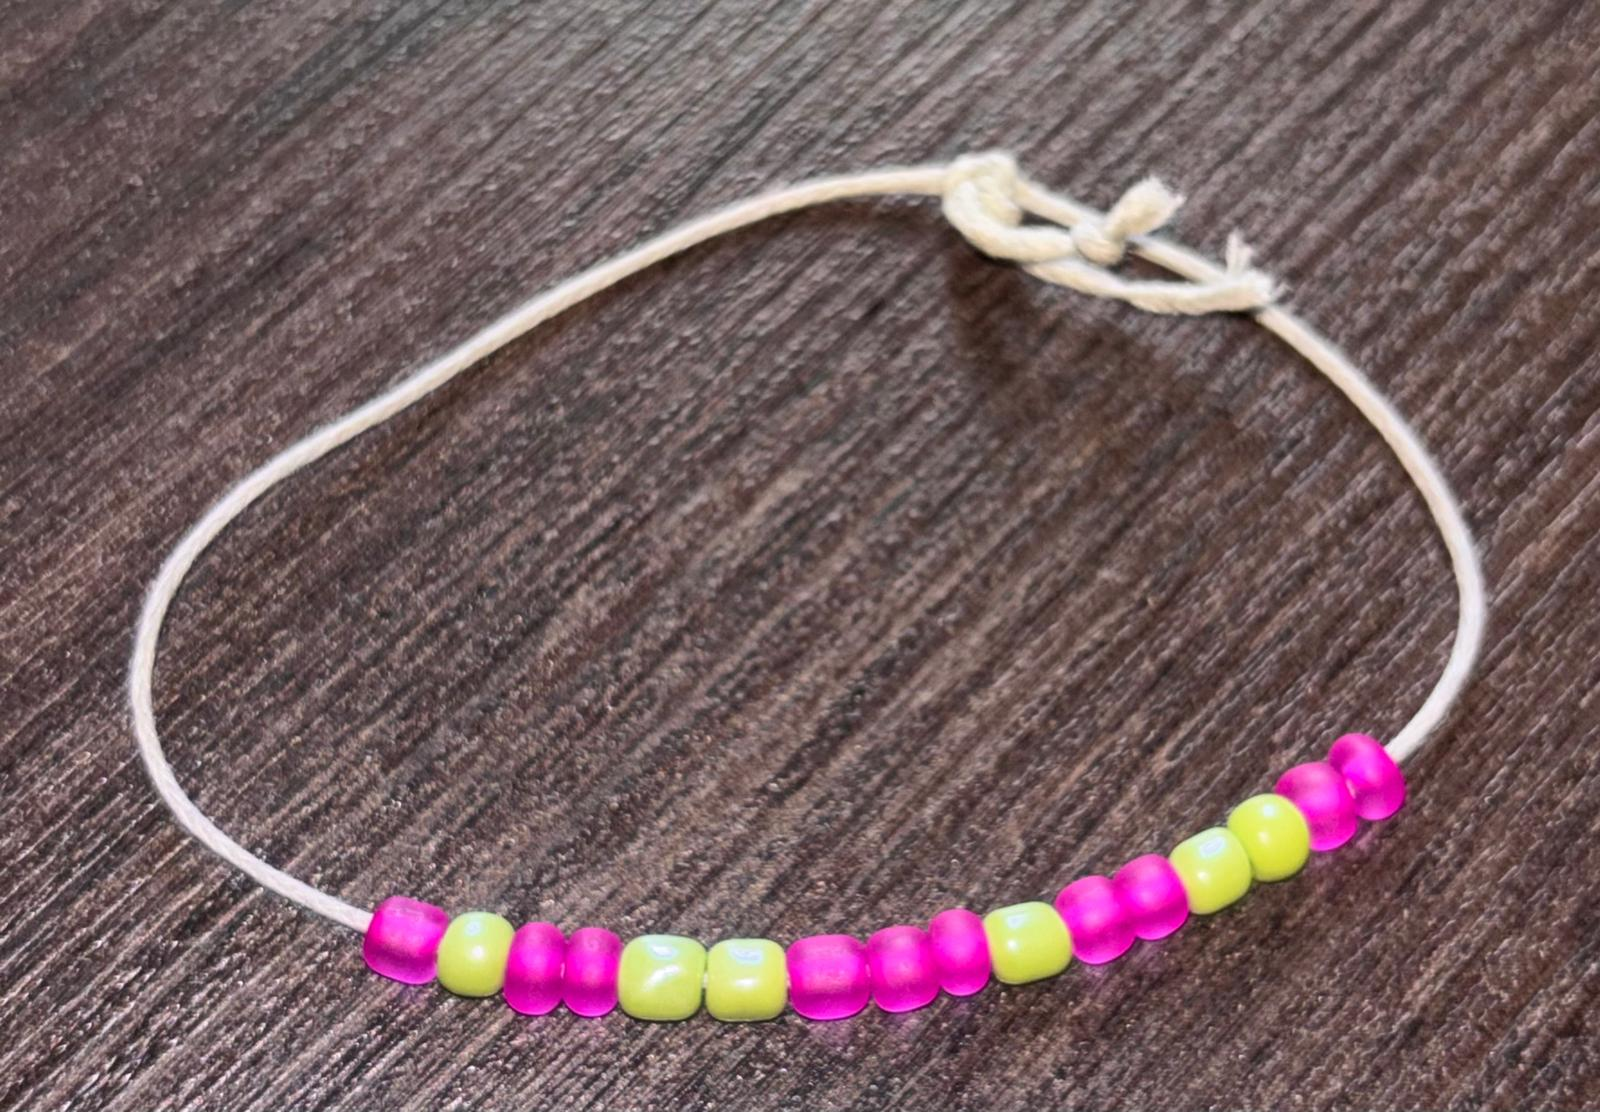
\includegraphics[scale=0.17]{bracciale.jpg}}
	\end{center}
\end{frame}

\section{\textbf{Insert a picture of your work}}
\begin{frame}{\textbf{Insert a picture of your work}}
	\begin{center}
		\zoombox{\includegraphics[scale=0.8]{example-image}}
	\end{center}
\end{frame}

\section{\textbf{License}}
\begin{frame}{\textbf{License}}
	\begin{center}
		\doclicenseThis
	\end{center}
\end{frame}
	
	
\end{document}